\nonstopmode

\documentclass[letterpaper,12pt,titlepage]{report}
\usepackage{amsthm,amssymb,mathtools}
\mathtoolsset{showonlyrefs}
\usepackage{bm}
\usepackage[margin=1in]{geometry}
\usepackage{booktabs}
\usepackage{enumitem}
\usepackage{framed}
\usepackage{tikz}
\usetikzlibrary{shapes,arrows,positioning,patterns,calc}
\usepackage{pgfplots}
\pgfplotsset{compat=1.9}

\usepackage{fancyhdr}
\pagestyle{fancy}
\fancyhead{}
\fancyfoot{}
\fancyfoot[L]{K.\ Okkelberg}
\fancyfoot[R]{\thepage}
\renewcommand{\headrulewidth}{0pt}
\renewcommand{\footrulewidth}{0.5pt}

\newcommand*\dif{\mathop{}\!\mathrm{d}}
\newcommand{\trans}{^\text{T}}
\newcommand{\herm}{^\text{H}}
\DeclareMathOperator{\E}{E}
\DeclareMathOperator{\trace}{trace}
\DeclareMathOperator{\sign}{sign}
\let\Pr\relax
\DeclareMathOperator{\Pr}{P}
\newcommand*\pder[2]{\frac{\partial #1}{\partial #2}}
\newcommand*\R{\mathbb{R}}

\theoremstyle{plain}
\newtheorem*{thm}{Theorem}
\theoremstyle{definition}
\newtheorem*{defi}{Definition}

\tikzstyle{line} = [draw, thick, >=latex]
\tikzstyle{dot} = [circle,fill=black,inner sep=0pt,minimum size=4pt]

\begin{document}

\title{ECE 6553: Optimal Control Notes}
\author{Klaus Z.\ Okkelberg}
\date{Spring 2017}
\maketitle

\chapter{Parameter Optimization}

% 2017/01/10
\section{What is optimal control?}
\paragraph{Optimal} Maximize/minimize cost (subject to constraints): $ \min_u g(u) $

With constraints,
\begin{align}
  \min_u {}\ & g(u) \\
  \text{s.t. } & \begin{cases} h_1(u) = 0 \\ h_2(u) \le 0 \end{cases}
\end{align}

First-order necessary condition (FONC):
\[ \frac{\partial g}{\partial u}(u^*) = 0 \]

Optimality can be
\begin{itemize}
\item local vs global
\item max vs min
\end{itemize}

\begin{center}
  \begin{tikzpicture}
    \draw [thick,->] (0,0) -- (0,4) node [anchor=east] {$g$};
    \draw [thick,->] (0,0) -- (6.5,0) node [anchor=north west] {$u$};
    \draw plot [smooth, tension=1] coordinates { (0.5,3) (2,0.5) (3.5,3) (4.25,1) (5,2) (5.5,1.5) (6,2) };
    \draw [thick] (2,0.1) -- (2,-0.1) node [anchor=north] {$u^*$};
  \end{tikzpicture}
\end{center}

\paragraph{Control} control design: pick $u$ such that specifications are satisfied:
\[ \dot{x} = f(x,u), \qquad \dot{x} = Ax + Bu, \]
where $x(t)\in\mathbb{R}^n$ is the state, $u(t)\in\mathbb{R}^m$ is the control, and $f(\cdot)$ is the dynamics.

Actually, $x$ and $u$ are signals:
\[ x:[0,T]\to\mathbb{R}^n, \qquad u:[0,T]\to\mathbb{R}^m \]

\paragraph{Optimal control} find the ``best'' u!

For ``best'' to mean anything, we need a cost. The big/deep question is
\[ \frac{\partial \text{``cost''}}{\partial u} = 0 \]

\paragraph{Example} \mbox{}

Suppose we have a car with position $p$. Its acceleration $\ddot{p}$ is controlled by the gas/brake input $u$ ($\ddot{p}=u$). In order to express the dynamics of the system in the form $\dot{x}=f(x,u)$, we introduce state variables:
\[
  \begin{aligned} x_1 &= p \\ x_2 &= \dot{p} \end{aligned}
  \ \Longrightarrow \
  \begin{cases} \dot{x}_1 = x_2 \\ \dot{x}_2 = u \end{cases}
\]
The task is to move the car from its initial position to a stop at a distance $c$ away.

\subparagraph{Minimum energy problem}
\begin{align}
  \min_u {}\ & \int_0^T\! u^2(t) \dif t \\
  \text{s.t. } & \begin{cases} \dot{x}_1 = x_2 \\ \dot{x}_2 = u \end{cases} \\
             & x_1(0) = 0,\, x_2(0) = 0 \\
             & x_1(T) = c,\, x_2(T) = 0
\end{align}

\subparagraph{Minimum time problem}
\begin{align}
  \min_{u,T} {}\ & T = \int_0^T\! \dif t \\
  \text{s.t. } & \begin{cases} \dot{x}_1 = x_2 \\ \dot{x}_2 = u \end{cases} \\
                 & x_1(0) = 0,\, x_2(0) = 0 \\
                 & x_1(T) = c,\, x_2(T) = 0 \\
                 & u(t) \in [u_\text{min},u_\text{max}]
\end{align}

The general optimal control problem we will solve will look like
\begin{align}
  \min_{u,T} {}\ & \int_0^T\! L(x(t),u(t),t) \dif t + \Psi(x(T)) \\
  \text{s.t. } & \dot{x}(t) = f(x(t),u(t),t),\ t\in[0,T] \\
                 & x(0) = x_0 \\
                 & x(T) \in S \\
                 & u(t) \in \Omega,\ t\in[0,T]
\end{align}
where $\Psi(\cdot)$ is the terminal cost and $S$ is the terminal manifold. This is a so-called \textbf{Bolza Problem}.

\paragraph{What tools do we need to solve this?}
\begin{enumerate}
\item optimality conditions $\partial\text{cost}/\partial u=0$
\item some way of representing the optimal signal $u^*(x,t)$
\item some way of actually finding/computing the optimal controllers
\end{enumerate}

% 2017/01/12
\section{Unconstrained Optimization}

Let the decision variable be $u=[u_1, \dots, u_m]\trans\in\mathbb R^m$. The cost is $g(u)\in C^1$ ($C^k$ means $k$ times continuously differentiable). The problem is
\[ \min_u g(u), \quad g:\mathbb R^m \to \mathbb R \]
For $u^*$ to be a minimizer, we need
\[ \pder{g}{u} (u^*) = 0 \]
\begin{defi}
$u^*$ is a (local) minimizer to $g$ if $\exists\delta>0$ s.t.
\begin{gather}
g(u^*) \le g(u) \quad \forall u\in B_\delta(u^*) \\
B_\delta(u^*) = \{ u \mid \Vert u-u^* \Vert \le \delta \}
\end{gather}
\end{defi}

\paragraph{Note:} \mbox{}
\begin{itemize}
\item $\displaystyle \pder{g}{u}(u^*) \delta u \in \mathbb R$ and $\delta u$ is $m\times 1$, so $\displaystyle \pder{g}{u}$ is a $1\times m$ row vector. For the column vector,
\[ \nabla g = \pder{g\trans}{u} \in \mathbb R^m \]
\item $\displaystyle \pder{g}{u} \, \delta u$ is an inner product
\[ \langle \nabla g, \delta u \rangle = \left\langle \pder{g\trans}{u}, \delta u \right\rangle \]
\item $o(\epsilon)$ encodes higher-order terms
\[ \lim_{\epsilon\to 0} \frac{o(\epsilon)}{\epsilon} = 0 \qquad \text{``faster than linear''} \]
This is opposed to big-O notation:
\[ \lim_{\epsilon\to 0} \frac{\mathcal O(\epsilon)}{\epsilon} = c \]
\item $\delta u$ has direction and scale so we could write it as
\[ \delta u = \epsilon v, \quad \epsilon\in\mathbb R,\ v\in\mathbb R^m \]
\end{itemize}

\begin{thm}
For $u^*$ to be a minimizer, we need
\[ \pder{g}{u} (u^*) = 0 \]
or, equivalently,
\[ \pder{g}{u} (u^*) v = 0 \quad \forall v\in\mathbb R^m \]
\end{thm}

\begin{proof}
Let $u^*$ be a minimizer. Evaluating the cost $g(u)$ in the ball and using Taylor's expansion,
\[ g(u^* + \delta u) = g(u^*) + \pder{g}{u} (u^*) \delta u + o(\Vert\delta u\Vert) = g(u^*) + \epsilon \pder{g}{u} (u^*) v + o(\epsilon) \]
Assume that $\pder{g}{u} \neq 0$. Then we could pick $v=-\pder{g\trans}{u}(u^*)$, i.e.
\[ g(u^*+\epsilon v) = g(u^*) - \epsilon \left\Vert \pder{g\trans}{u} (u^*) \right\Vert^2 + o(\epsilon) \]
Note that the second term is negative per our assumptions. So, for $\epsilon$ sufficiently small, we have
\[ g \Big( u^* - \epsilon\pder{g\trans}{u} (u^*) \Big) < g(u^*) \]
This contradicts $u^*$ being a minimizer. \quad

\begin{tikzpicture}[scale=0.3]
  \draw (0,0) -- (1,1);
  \draw (0,1) -- (1,0);
  \draw (0,0.35) -- (0.35,0);
  \draw (0.65,0) -- (1,0.35);
\end{tikzpicture}
(crossed swords)
\end{proof}

\begin{defi}[Positive definite]
$M=M\trans \succ 0$ if
\begin{gather}
  z\trans M z > 0 \quad \forall z\neq 0,\ z\in\mathbb R^m \\
  \Longleftrightarrow M \text{ has real and positive eigenvalues}
\end{gather}
\end{defi}

\begin{thm}
If $g\in C^2$, then a \textbf{sufficient} condition for $u^*$ to be a (local) minimizer is
\begin{enumerate}
\item $\displaystyle \pder{g}{u}(u^*) = 0$
\item $\displaystyle \pder{^2 g}{u^2}(u^*) \succ 0$ (the Hessian is positive definite)
\end{enumerate}
\end{thm}

\begin{defi}
$g:\mathbb R^m\to\mathbb R$ is convex if
\[ g(\alpha u_1 + (1-\alpha)u_2) \le \alpha g(u_1) + (1-\alpha)g(u_2) \quad \forall \alpha\in[0,1], \ u_1,\! u_2\in\mathbb R^m \]
\begin{center}
  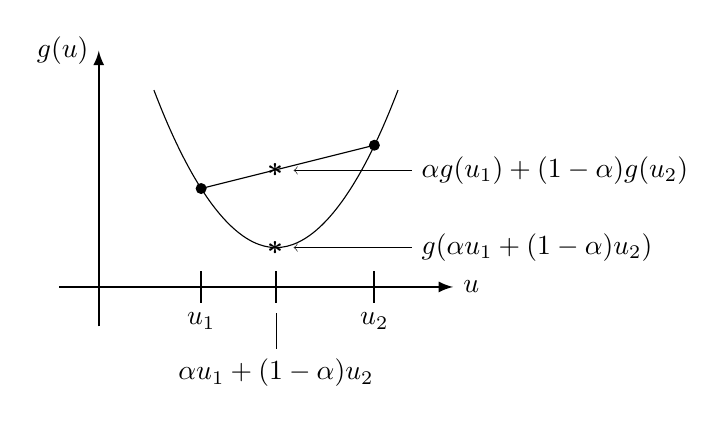
\begin{tikzpicture}
    \path [line,->] (-0.5,0) -- (4.5,0) node [anchor=west] {$u$};
    \path [line,->] (0,-0.5) -- (0,3) node [anchor=east] {$g(u)$};
    \draw (0.7,2.5) parabola bend (2.25,0.5) (3.8,2.5);
    \path [line] (1.3,-0.2) node [anchor=north] {$u_1$} -- (1.3,0.2);
    \path [line] (3.5,-0.2) node [anchor=north] {$u_2$} -- (3.5,0.2);
    \path [line] (2.25,-0.2) node [pin={[pin edge={black}] below:{$\alpha u_1 + (1-\alpha)u_2$}}] {} -- (2.25,0.2);
    \draw (1.3,1.25) -- (3.5,1.8);
    \fill (1.3,1.25) circle (0.07);
    \fill (3.5,1.8) circle (0.07);
    \node [pin={[pin edge={black,<-},pin distance=1.5cm] right:{$g(\alpha u_1 + (1-\alpha)u_2)$}}] at (2.25,0.5) {$\bm *$};
    \node [pin={[pin edge={black,<-},pin distance=1.5cm] right:{$\alpha g(u_1) + (1-\alpha)g(u_2)$}}] at (2.25,1.48) {$\bm *$};
  \end{tikzpicture}
\end{center}
\end{defi}

\begin{thm}
If $\pder{^2 g}{u^2} (u) \succeq 0$ $\forall u\in\mathbb R^m$, then $g$ is convex. ($\Longleftrightarrow$ for $g\in C^2$)
\end{thm}

\paragraph{Example} $\displaystyle \min_u u\trans Q u - b\trans u$ where $Q=Q\trans\succ 0$ (positive definite matrix)
\begin{align}
\pder{g}{u} &= \pder{}{u} (u\trans Qu - b\trans u) \\
&= u\trans Q\trans + u\trans Q - b\trans \\
&= 2u\trans Q - b\trans \\[-3ex]
  \pder{^2 g}{u^2} &= 2Q
& \pder{^2 g}{u^2} = \begin{bmatrix}
  \pder{^2 g}{u_1^2} & \cdots & \pder{^2 g}{u_1 \partial u_m} \\
  \vdots & \ddots & \vdots \\
  \pder{^2 g}{u_m \partial u_1} & \cdots & \pder{^2 g}{u_m^2}
\end{bmatrix}
\end{align}
From $\pder{g}{u} = 2u\trans Q-b\trans = 0$,
\[ u = \frac12 Q^{-1} b \]
To see whether this is a minimizer, consider the Hessian. Since $Q \succ 0$, it follows that $\pder{^2 g}{u^2} (u^*) \succ 0$ and $u^*=\frac12 Q^{-1} b$ is a (local) minimizer. Additionally, since $\pder{^2 g}{u^2} \succ 0$, $g$ is convex and $u^*$ is a global minimizer. In fact, since we have strict convexity ($\succ 0$ rather than $\succeq 0$), it is the unique global minimizer.

In optimal control, \emph{local} is typically all we can ask for. In optimization, we can do better!

But wait, just because we know $\pder{g}{u}=0$, it doesn't follow that we can actually find $u^*$\dots

\section{Numerical Methods}
Idea: $u_{k+1}=u_k+\text{step}_k$. What should $\text{step}_k$ be? For small $\text{step}_k=\gamma_k v_k$,
\[ g(u_k \cdot \text{step}_k) = g(u_k) + \pder{g}{u}(u_k) \cdot \text{step}_k + o(\Vert \text{step}_k \Vert) = g(u_k) + \gamma_k \pder{g}{u}(u_k) v_k + o(\gamma_k) \]
A perfectly reasonable choice of step direction is
\[ v_k=-\pder{g\trans}{u}(u_k), \]
known as the \emph{steepest descend} direction. This produces
\[ g \Big( u_k - \gamma_k\pder{g}{u}(u_k) \Big) = g(u_k) - \gamma_k \left\Vert \pder{g}{u}(u_k) \right\Vert^2 + o(\gamma_k) \]

\begin{framed}
  \textbf{Steepest descent} \[ u_{k+1} = u_k - \gamma_k \pder{g\trans}{u} (u_k) \]
\end{framed}

\paragraph{Note:} \mbox{}
\begin{itemize}
\item What should $\gamma_k$ be?
\item This method ``pretends'' that $g(u)$ is linear. If we pretend $g(u)$ is quadratic, we get
  \[ u_{k+1} = u_k - \left( \pder{^2 g}{u^2} (u_k) \right)^{-1} \pder{g\trans}{u} (u_k), \]
  i.e.\ Newton's Method
\end{itemize}

\paragraph{This course:} steepest descent

\subparagraph{Step-size selection?} \mbox{}
\begin{itemize}
\item Choice 1: $\gamma_k=\gamma$ ``small'' $\forall k$; will get close to a minimizer if $u_0$ is close enough and $\gamma$ small enough

  Problems: \vspace{-1ex}
  \begin{itemize}
  \item You may not converge! (but you'll get close)
  \item You may go off to infinity (diverge)
  \end{itemize}

  \begin{center}
    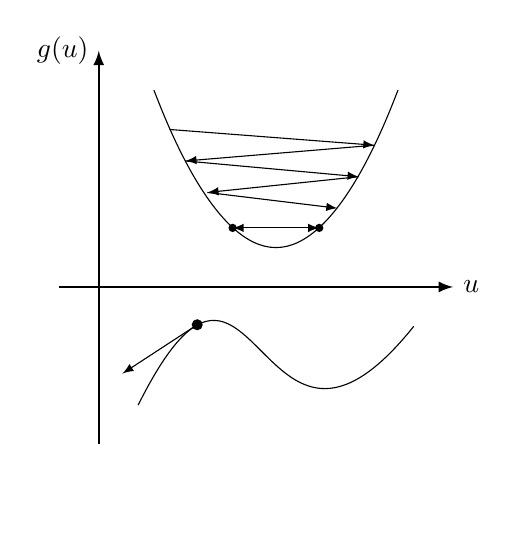
\begin{tikzpicture}
      \path [line,->] (-0.5,0) -- (4.5,0) node [anchor=west] {$u$};
      \path [line,->] (0,-2) -- (0,3) node [anchor=east] {$g(u)$};
      \draw (0.7,2.5) parabola bend (2.25,0.5) (3.8,2.5);
      \draw (0.5,-1.5) .. controls (2,1.5) and (2,-3) .. (4,-0.5);

      \draw [<->,>=latex] (1.7,0.75) node [circle,fill=black,minimum size=3pt,inner sep=0pt] {} -- (2.8,0.75) node [circle,fill=black,minimum size=3pt,inner sep=0pt] {};

      \draw [->,>=latex] (0.9,2) -- (3.5,1.8);
      \draw [->,>=latex] (3.5,1.8) -- (1.1,1.6);
      \draw [->,>=latex] (1.1,1.6) -- (3.3,1.4);
      \draw [->,>=latex] (3.3,1.4) -- (1.38,1.2);
      \draw [->,>=latex] (1.38,1.2) -- (3.03,1);

      \draw [->,>=latex] (1.25,-0.48) node [circle,fill=black,inner sep=0pt,minimum size=4pt] {} -- (0.3,-1.1);
    \end{tikzpicture}
  \end{center}
  
\item Choice 2: Reduce $\gamma_k$ as a function of $k$; will get close to a minimizer if $u_0$ is close enough

  Problem: slow

  \begin{thm}
    If $u_0$ is close enough to $u^*$ and $\gamma_k$ satisfies
    \begin{itemize}
    \item $\displaystyle \sum_{k=0}^\infty \gamma_k = \infty$
    \item $\displaystyle \sum_{k=0}^\infty \gamma_k^2 < \infty$
    \end{itemize}
    e.g.\ $\gamma_k=c/k$, then $u_k\to u^*$ as $k\to\infty$.
  \end{thm}
  
% 2017/01/17
\item Choice 3: \textbf{Armijo step-size:} Take as big a step as possible, but no larger

  Pick $\alpha\in(0,1)$, $\beta\in(0,1)$. Let $i$ be the smallest non-negative integer such that
  \begin{gather}
    g\left( u_k - \beta^i \pder{g\trans}{u}(u_k) \right) - g(u_k) < -\alpha\beta^i \left\Vert \pder{g}{u}(u_k) \right\Vert^2 \\
    u_{k+1} = u_k - \beta^i \pder{g\trans}{u}(u_k)
  \end{gather}
  This will get to a minimizer blazingly fast if $u_0$ is close enough.
\end{itemize}

\section{Constrained Optimization}

Equality constraints:
\begin{align}
  \min_{u\in\mathcal R^m} {}\ & g(u) \\
  \text{s.t. } & h(u)=\bm 0
\end{align}
Consider $u\in\mathbb R^2$, $h:\mathbb R^2\to\mathbb R$
\begin{center}
  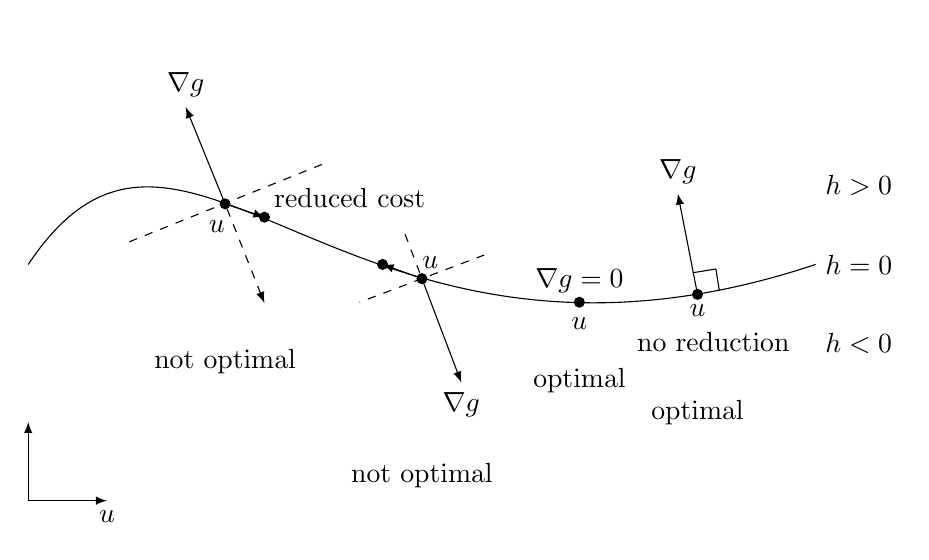
\begin{tikzpicture}[>=latex]
    \draw (0,0) .. controls (2,3) and (4,-2) .. (10,0) node [anchor=west] {$h=0$};
    \draw [>=latex,->] (0,-3) -- (0,-2);
    \draw [>=latex,->] (0,-3) -- (1,-3) node [anchor=north] {$u$};
    \node [anchor=west] at (10,1) {$h>0$};
    \node [anchor=west] at (10,-1) {$h<0$};

    \path
    coordinate (u) at (2.5,0.77)
    coordinate  (A) at (2,2)
    coordinate (B) at (3,-0.49)
    coordinate (C) at ($(u)!1!-90:(A)$)
    coordinate (D) at ($(A)!(C)!(B)$)
    coordinate (rc) at (3,0.6);
    \draw [->] (u) node [dot] {} -- (A) node [anchor=south] {$\nabla g$};
    \draw [<-,dashed] (B) -- (u) node [anchor=north,inner sep=6pt,xshift=-3pt] {$u$};
    \draw [dashed] (C) -- ($(C)!2!(D)$);
    \draw [->] (u) -- (rc) node [anchor=south west] {reduced cost};
    \node [circle,fill=black,inner sep=0pt,minimum size=4pt] at (rc) {};
    \node at ($(u)-(0,2)$) {not optimal};

    \draw [->]  (5,-0.18) node [dot] (u2) {} -- (5.5,-1.5) coordinate (A2);
    \node [anchor=north] at (A2) {$\nabla g$};
    \draw [dashed] (u2) node [anchor=south,xshift=3pt] {$u$} -- ($(A2)!1.5!(u2)$);
    \draw [dashed] ($(u2)!0.6!90:(A2)$) -- ($(u2)!0.6!-90:(A2)$);
    \draw [->] (u2) -- (4.5,-0) node [dot] {};
    \node at ($(u2)-(0,2.5)$) {not optimal};

    \node [dot] (u3) at (7,-0.48) {};
    \node [anchor=south] at (u3) {$\nabla g=0$};
    \node [anchor=north,yshift=-2pt] at (u3) {$u$};
    \node at ($(u3)-(0,1)$) {optimal};

    \draw [->] (8.5,-0.38) node [dot] (u4) {} -- (8.25,0.9) node [anchor=south] (A4) {$\nabla g$};
    \draw [shorten <=-0.5pt] ($(u4)!8pt!(A4)$) coordinate (B4) -- ($(B4)!1!90:(u4)$) coordinate (C4);
    \draw (C4) -- ($(C4)!1!90:(B4)$);
    \node [anchor=north] at (u4) {$u$};
    \node at ($(u4)-(-0.2,0.6)$) {no reduction};
    \node at ($(u4)-(0,1.5)$) {optimal};
  \end{tikzpicture}
\end{center}
So $u$ is (locally) optimal if $\nabla g \parallel$ (is parallel to) the normal vector to tangent plane to h.

\medskip
Fact: (HW\# 1)
\[ \nabla h \perp Th \quad \text{(tangent plane to h)} \]
\begin{center}
  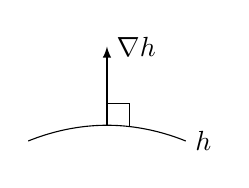
\begin{tikzpicture}
    \coordinate (u) at (1,0.2);
    \draw (0,0) parabola bend (u) (2,0) node [anchor=west] {$h$};
    \draw [->,>=latex] (u) -- ($(u)+(0,1)$) node [anchor=west] {$\nabla h$};
    \draw ($(u)+(0,8pt)$) coordinate (b) -- ($(b)!1!90:(u)$) coordinate (c);
    \draw [shorten >=-0.5pt] (c) -- ($(c)!1!90:(b)$);
  \end{tikzpicture}
\end{center}
We need $\nabla g \parallel \nabla h$ at $u^*$ for optimality, i.e.
\[ \pder{g}{u}(u^*) = \alpha \pder{h}{u}(u^*), \quad \text{for some } \alpha\in\R \]
or ($\lambda=-\alpha$),
\[ \pder{g}{u}(u^*) + \lambda \pder{h}{u}(u^*) = 0 \]
or
\[ \pder{}{u} \big( g(u^*) + \lambda h(u^*) \big) = 0, \quad \text{for some } \lambda\in\R \]
More generally,
\begin{align}
  \min_{u\in\mathcal R^m} {}\ & g(u) \\
  \text{s.t. } & h(u)=\bm 0, \quad h:\R^m\to\R^k
\end{align}
Note that $h(u)=[h_1(u),\dots,h_k(u)]\trans$.

We need $\pder{g}{u}(u^*)$ to be a linear combination of $\pder{h_i}{u}(u^*)$, $i=1,\dots,k$, for exactly the same reasons, i.e.
\[ \pder{g}{u}(u^*) = \sum_{i=1}^k \alpha_i \pder{h_i}{u}(u^*) \]
or ($\lambda=-[\alpha_1,\dots,\alpha_k]\trans$)
\[ \pder{g}{u}(u^*) + \lambda\trans \pder{h}{u}(u^*) = 0 \]
or
\[ \pder{}{u} \big( g(u^*) + \lambda\trans h(u^*) \big) = 0, \quad \text{for some } \lambda\in\R^k \]

\begin{thm}
  If $u^*$ is a minimizer to 
  \begin{align}
    \min_{u\in\mathcal R^m} {}\ & g(u) \\
    \text{s.t. } & h(u)=\bm 0, \quad h:\R^m\to\R^k
  \end{align}
  then $\exists\lambda\in\R^k$ s.t.
  \[ \begin{cases}
    \displaystyle \pder{L}{u}(u^*,\lambda) = 0 \\[2ex]
    \displaystyle \pder{L}{\lambda}(u^*,\lambda) = 0
  \end{cases} \]
  where the Lagrangian $L$ is given by
  \[ L(u,\lambda) = g(u) + \lambda\trans h(u) \]
\end{thm}

\paragraph{Note:}
\begin{itemize}
\item $\lambda$ are the Lagrange multipliers
\item $\pder{L}{\lambda}=0$ is fancy speak for $h(u^*)=0$
\end{itemize}

\paragraph{Example}
\begin{align}
  \min_{u\in\R^m} {}\ & \frac12 \Vert u\Vert^2 \\
  \text{s.t. } & Au=b
\end{align}
where $A$ is $k\times m$, $k\le m$. Assume $(AA\trans)^{-1}$ exists (constraints are linearly independent, none of the constraints are ``duplicates'', all the constraints are essential).
\begin{align}
  L &= \frac12 u\trans u + \lambda\trans (Au-b) \\
  \pder{L}{u} &= u\trans + \lambda\trans A = 0 \\
  u^* &= -A\trans \lambda \\
  \shortintertext{Using the equality constraint,}
  A u^* &= b \\
  -A A\trans \lambda &= b \\
  \lambda &= -(AA\trans)^{-1} b \\
  u^* &= A\trans (AA\trans)^{-1} b
\end{align}

\paragraph{Example}
\begin{align}
  \min {}\ & u_1u_2 + u_2u_3 + u_1u_3 \\
  \text{s.t. } & u_1 + u_2 + u_3 = 3
\end{align}
\[ L = u_1u_2 + u_2u_3 + u_1u_3 + \lambda (u_1 + u_2 + u_3 - 3) \]
\begin{align}
  \begin{cases}
    \pder{L}{u_1} = u_2 + u_3 + \lambda = 0 \\
    \pder{L}{u_2} = u_1 + u_3 + \lambda = 0 \\
    \pder{L}{u_3} = u_2 + u_1 + \lambda = 0 \\
    \pder{L}{\lambda} = u_1 + u_2 + u_3 = 3
  \end{cases}
  \Longrightarrow
  \begin{cases}
    u_1^* = 1 \\
    u_2^* = 1 \\
    u_3^* = 1 \\
    \lambda = -2
  \end{cases}
  \quad \text{optimal solution}
\end{align}
Note: This was actually the worst we can do---maximize! Even weirder: no local minimizer!

% 2017/01/19
\subsection{Equality Constraints}
\begin{align}
  \min_{u\in\mathcal R^m} {}\ & g(u) \\
  \text{s.t. } & h(u)=\bm 0, \quad h:\R^m\to\R^k
\end{align}
\begin{thm}
  If $u^*$ is a minimizer/maximizer then $\exists\lambda\in\R^k$ s.t.
  \begin{align}
    \pder{L}{u}(u^*,\lambda) &= 0 \\
    \pder{L}{\lambda}(u^*,\lambda) &= 0 \qquad (\Longleftrightarrow h(u^*)=0)
  \end{align}
  where $L(u,\lambda) = g(u) + \lambda\trans h(u)$.
\end{thm}

\paragraph{Example} [Entropy Maximization]

Given $S=\{x_1,\dots,x_n\}$ and a distribution over $S$ such that it takes the value $x_j$ with probability $p_j$. The entropy is
\[ E(p) = \sum_{j=1}^n (-p_j \ln p_j). \]
The mean is
\[ m = \sum_{j=1}^n p_jx_j. \]
Problem: Given $m$, find $p$ such that $E$ is maximized.
\begin{align}
  \min_{p} {}\ & -\sum_{j=1}^n p_j \ln p_j \\
  \text{s.t. } & \sum_{j=1}^n p_j x_j = m \\
               & \sum_{j=1}^n p_j = 1 \\
               & p_j \ge 0, \ j=1,\dots,n \quad \text{(ignore this\dots)}
\end{align}
\begin{align}
  L &= - \sum p_j \ln p_j + \lambda_1 \left[ \sum p_j x_j -m \right] + \lambda_2 \left[ \sum p_j - 1 \right] \\
  \pder{L}{p_j} &= -\ln p_j - 1 + \lambda_1 x_j + \lambda_2 = 0 \\
  p_j &= e^{\lambda_2 - 1 + \lambda_1 x_j}, \quad j=1,\dots,n \qquad (p_j\ge0 \text{ so we're ok with ignoring that})
\end{align}
\begin{align}
\sum e^{\lambda_2 - 1 + \lambda_1 x_j} x_j &= m && n+2 \text{ equations and} \\
  \sum e^{\lambda_2 - 1 + \lambda_1 x_j} &= 1 && n+2 \text{ unknowns\dots}
\end{align}
No analytical solution, but numerically ``solvable''

\subsection{Inequality Constraints}
\begin{align}
  \min_{u\in\mathcal R^m} {}\ & g(u) \\
  \text{s.t. } & h(u)\le\bm 0, \quad h:\R^m\to\R^k
\end{align}
\begin{center}
  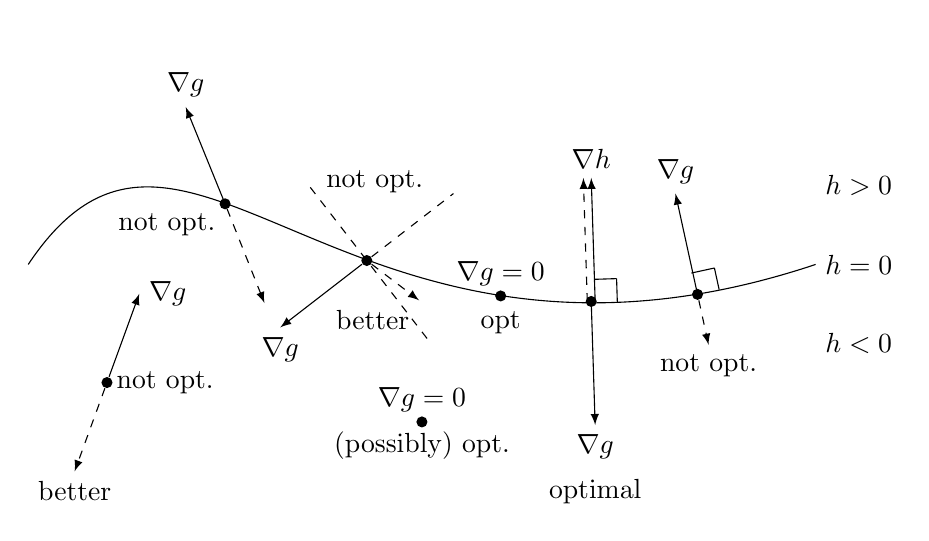
\begin{tikzpicture}[>=latex]
    \draw (0,0) .. controls (2,3) and (4,-2) .. (10,0) node [anchor=west] {$h=0$};
    \node [anchor=west] at (10,1) {$h>0$};
    \node [anchor=west] at (10,-1) {$h<0$};

    \path
    coordinate (u) at (2.5,0.77)
    coordinate  (A) at (2,2)
    coordinate (B) at (3,-0.49);
    \draw [->] (u) node [dot] {} -- (A) node [anchor=south] {$\nabla g$};
    \draw [<-,dashed] (B) -- (u) node [anchor=north east] {not opt.};

    \node [dot] (u3) at (6,-0.40) {};
    \node [anchor=south] at (u3) {$\nabla g=0$};
    \node [anchor=north,yshift=-2pt] at (u3) {opt};

    \coordinate (u2) at (7.2,-0.47);
    \coordinate (A2) at (7.15, 1.1);
    \draw [->] (u2) -- (A2) node [anchor=south] {$\nabla h$};
    \draw [->] ($(u2)+(-0.05,0)$) node [dot] {} -- ($(u2)!-1!(A2)+(-0.05,0)$) node [anchor=north] (D2) {$\nabla g$};
    \draw ($(u2)!8pt!(A2)$) coordinate (B2) -- ($(B2)!1!90:(u2)$) coordinate (C2);
    \draw [shorten >=-0.5pt] (C2) -- ($(C2)!1!90:(B2)$);
    \draw [->,dashed] ($(u2)+(-0.1,0)$) -- ($(A2)+(-0.1,0)$);
    \node [anchor=north,yshift=-8pt] at (D2) {optimal};

    \draw [->] (8.5,-0.38) node [dot] (u4) {} -- (8.22,0.9) coordinate (A4);
    \node [anchor=south] at (A4) {$\nabla g$};
    \draw [->,dashed] (u4) -- ($(u4)!-0.5!(A4)$) node [anchor=north] {not opt.};
    \draw [shorten <=-0.5pt] ($(u4)!8pt!(A4)$) coordinate (B4) -- ($(B4)!1!90:(u4)$) coordinate (C4);
    \draw (C4) -- ($(C4)!1!90:(B4)$);

    \node [dot] (u5) at (4.3,0.05) {};
    \draw [->] (u5) -- (3.2,-0.8) coordinate (a5);
    \node [anchor=north] at (a5) {$\nabla g$};
    \draw [dashed] (u5) -- ($(u5)!-1!(a5)$) coordinate (b5);
    \draw [dashed] ($(u5)!0.9!90:(a5)$) -- ($(u5)!0.9!90:(b5)$);
    \draw [->,dashed] (u5) -- ($(u5)!0.6!-75:(b5)$) node [anchor=north east] {better};
    \node at ($(u5)+(0.1,1)$) {not opt.};

    \node [dot] (u6) at (5,-2) {};
    \node [anchor=south] at (u6) {$\nabla g=0$};
    \node [anchor=north] at (u6) {(possibly) opt.};

    \node [dot] (u7) at (1,-1.5) {};
    \draw [->] (u7) -- +(70:1.2) coordinate (a7);
    \node [anchor=west] at (a7) {$\nabla g$};
    \draw [->,dashed] (u7) -- ($(u7)!-1!(a7)$) node [anchor=north] {better};
    \node [anchor=west] at (u7) {not opt.};
  \end{tikzpicture}
\end{center}

We need:
\begin{itemize}
\item if $h(u^*)<0$ then $\pder{g}{u}(u^*)=0$
\item if $h(u^*)=0$ then we need either
  \begin{gather}
    \pder{g}{u}(u^*) = 0 \\
    \shortintertext{or}
    \pder{g}{u}(u^*) = -\lambda\pder{h}{u}(u^*) \quad \text{for } \lambda>0
  \end{gather}
\end{itemize}
Or, even better,
\[ \pder{}{u} \left( g(u^*) + \lambda h(u^*) \right) = 0 \quad \text{for } \lambda\ge 0, \]
where $\lambda h(u^*)=0$. ($h<0\to\lambda=0$, $h=0\to\lambda\ge0$)

In general, if $u\in\R^m$ and $h:\R^m\to\R^k$, we have that $u^*$, if optimal, has to satisfy
\begin{gather}
  \pder{}{u} L(u^*,\lambda) = 0 \\
  h(u^*) \le \bm 0 \\
  \lambda\trans h(u^*) = 0 \\
  \lambda \ge \bm 0
\end{gather}
where the Lagrangian is $L(u,\lambda) = g(u) + \lambda\trans h(u)$. Note that if we're maximizing, the same holds except we need $\lambda\le 0$.

\paragraph{Example}
\begin{align}
  \min {}\ & 2u_1^2 + 2u_1u_2 + u_2^2 - 10u_1 - 10u_2 \\
  \text{s.t. } & \begin{cases}
    u_1^2 + u_2^2 \le 5 \\
    3u_1 + u_2 \le 6
  \end{cases}
\end{align}
\[ L = 2u_1^2 + 2u_1u_2 + u_2^2 - 10u_1 - 10u_2 + \lambda_1 (u_1^2 + u_2^2 - 5) + \lambda_2 (3u_1+u_2 - 6) \]
FONC:
\begin{enumerate}[label=\roman*)]
\item $\partial L/\partial u_1 = 4u_1 + 2u_2 - 10 + 2\lambda_1u_1 + 3\lambda_2$
\item $\partial L/\partial u_2 = 2u_1 + 2u_2 - 10 + 2\lambda_1u_2 + \lambda_2$
\item $u_1^2 + u_2^2 \le 5$
\item $3u_1 + u_2 \le 6$
\item $\lambda_1(u_1^2 + u_2^2 - 5) = 0$
\item $\lambda_2(3u_1 + u_2 - 6) = 0$
\item $\lambda_1 \ge 0$
\item $\lambda_2 \ge 0$
\end{enumerate}
To solve, assume different constraints are active/inactive:
\begin{enumerate}
\item Both constraints are inactive ($u_1^2 + u_2^2 < 5$, $3u_1 + u_2 < 6$) $\Longrightarrow \lambda_1=\lambda_2=0$
  \[ \begin{cases}
      4u_1 + 2u_2 - 10 = 0 \\
      2u_1 + 2u_2 - 10 = 0
    \end{cases}
    \Longrightarrow
    \begin{cases}
      u_1 = 0 \\
      u_2 = 5
    \end{cases} \]
  Note: iii) $0^2 + 5^2 \nleq 5$

  Not feasible

\item Assume constraint 1 is active and constraint 2 is inactive ($u_1^2 + u_2^2 = 5$, $\lambda_2=0$)
  \[ \begin{cases}
      4u_1 + 2u_2 - 10 + 2\lambda_1u_1 = 0 \\
      2u_1 + 2u_2 - 10 + 2\lambda_1u_2 = 0 \\
      u_1^2 + u_2^2 = 5
    \end{cases}
    \Longrightarrow
    \begin{cases}
      u_1 = 1 \\
      u_2 = 2 \\
      \lambda_1 = 1
    \end{cases} \]
  \begin{enumerate}[label=$\square$\hspace{1pt}\llap{\protect\raisebox{2pt}{$\checkmark$}}]
  \item $\lambda_1 \ge 0$
  \item $3\cdot 1 + 2 \le 6$
  \end{enumerate}
  This is a local minimizer

\item Assume constraint 2 is active and constraint 1 is inactive
\item Assume both constraints are active
\end{enumerate}

\paragraph{Kuhn-Tucker Conditions} (KKT conditions, Karush-Kuhn-Tucker)
\subparagraph{Problem:}
\begin{equation}
  \begin{aligned}
    \min_{u\in\R^m} {}\ & g(u) \\
    \text{s.t. } & \begin{cases}
      h_1(u) = 0, & h_1:\R^m\to\R^p \\
      h_2(u) \le 0, & h_2:\R^m\to\R^k
    \end{cases}
  \end{aligned}
  \label{eq:kkt}
\end{equation}

\begin{thm}
  Let $u^*$ be feasible ($h_1=0$, $h_2\le0$). If $u^*$ is a minimizer to \eqref{eq:kkt} than there exists vectors $\lambda\in\R^p$, $\mu\in\R^k$ with $\mu\ge\bm 0$ such that
  \[ \begin{cases}
      \displaystyle \pder{g}{u}(u^*) + \lambda\trans \pder{h_1}{u}(u^*) + \mu\trans \pder{h_2}{u}(u^*) = 0 \\[1ex]
      \mu\trans h_2(u^*) = 0
    \end{cases} \]
\end{thm}

Looking ahead: $\min \text{cost}(u(\cdot))$ s.t.\ $\dot x = f(x,u)$ (dynamics), where $u$ is a function. Note the equality constraint

% 2017/01/24
\paragraph{Question:} How do we go from $u\in\R^m$ to $u\in\mathcal U$ (function space)?
\subparagraph{Note:} Function space is a set of functions of a given kind from a set $X$ to a set $Y$
\begin{enumerate}
\item linear function
\item square-integrable functions: $L_2[0,T]:$ $\int_0^T \Vert u(t)\Vert^2 \dif t < \infty$
\item $C^\infty (\R)$
\end{enumerate}
What would $\partial \text{``cost''}/\partial u$ mean?

\section{Directional Derivatives}
\paragraph{Recall:} To minimize $g(u)$, let $u^*$ be a candidate minimizer and pitch a perturbation on $u^*$

\begin{gather}
  g(u^* + \epsilon v) = g(u^*) + \epsilon \pder{g}{u}(u^*) v + o(\epsilon) \\
  \text{FONC: } \pder{g}{u}(u^*) = 0 \hspace{3cm} 
\end{gather}

\subparagraph{Note:} $\pder{g}{u}(u^*) v$ tells us how much $g(u)$ increases/decreases in the direction of $v$.

\begin{defi}
  The directional (Gateaux) derivative is given by
  \[ \delta g(u;v) = \lim_{\epsilon\to0} \frac{g(u+\epsilon v)-g(u)}{\epsilon} \]
\end{defi}

\paragraph{Example}
\[ g(u) = \frac12 u_1^2 - u_1 + 2u_2, \quad g:\R^2\to\R \]
Let's consider $e_1=[1\ 0]\trans$, $e_2=[0\ 1]\trans$. What is $\delta g(u;e_i)$, $i=1,2$?
\begin{align}
  \delta g(u;v) &= \lim_{\epsilon\to0} \frac{g(u+\epsilon v)-g(u)}{\epsilon} \\
                &= \lim_{\epsilon\to0} \frac{g(u)+\epsilon\pder{g}{u}(u) v + o(\epsilon) - g(u)}{\epsilon} \\
                &= \pder{g}{u} (u) v
\end{align}
\begin{align}
  \pder{g}{u}(u) &= [u_1-1\ 2] \\
  \delta g(u;e_1) &= [u_1-1\ 2] e_1 = u_1-1 \\
  \delta g(u;e_2) &= [u_1-1\ 2] e_2 = 2 \\
\end{align}

But the beauty of directional derivatives is that they generalize beyond vectors, $u\in\R^m$, to function spaces ($\mathcal U$) or other ``objects'' like matrices.

\paragraph{Example} $M\in\R^{n\times n}$, $F(M)=M^2$

What is $\pder{F}{M}$? (ponder at home\dots)

We can easily compute $\delta F(M;N)$!
\begin{align}
  F(M+\epsilon N) &= (M+\epsilon N)(M+\epsilon N) = M^2 + \epsilon M N + \epsilon N M + \epsilon^2 N^2 \\
  \delta F(M;N) &= \lim_{\epsilon\to0} \frac{F(M+\epsilon N)-F(M)}{\epsilon} \\
                  &= \lim_{\epsilon\to0} \frac{\epsilon M N + \epsilon N M + \epsilon^2 N^2}{\epsilon} = MN + NM
\end{align}

\paragraph{Infinite Dimensional Optimization}
Let $u\in\mathcal U$ (function space) and let $J(u)$ be the cost:
\[ \min_{u\in\mathcal U} J(u) \]

\begin{thm}
  If $u^*\in\mathcal U$ is a (local) minimizer then
  \[ \delta J(u^*;v) = 0, \quad \forall v\in\mathcal U \]
\end{thm}

\paragraph{Example} Find minimizer $u^*$ to
\[ J(u) = \int_0^T L(u(t)) \dif t \]
\begin{align}
  J(u+\epsilon v) - J(u) &= \int_0^T L(u(t)+\epsilon v(t)) \dif t - \int_0^T L(u(t)) \dif t, \quad u,v\in\mathcal U \\
                         &= \int_0^T \left[ L(u(t)) + \epsilon \pder{L}{u}(u(t)) v(t) + o(\epsilon) - L(u(t)) \right] \dif t \\
  \delta J(u^*;v) &= \lim_{\epsilon\to0} \frac{J(u+\epsilon v)-J(u)}{\epsilon} \\
                         &= \lim_{\epsilon\to0} \frac{\int_0^T \epsilon \pder{L}{u}(u(t)) v(t) \dif t + o(\epsilon)}{\epsilon} \\
                         &= \int_0^T \pder{L}{u}(u(t)) v(t) \dif t \\
\end{align}
$u^*$ optimizer:
\begin{gather}
  \delta J(u^*;v) = \int_0^T \pder{L}{u}(u(t)) v(t) \dif t = 0 \quad \forall v\in\mathcal U \\
  \Updownarrow \\
  \pder{L}{u} (u(t)) = 0 \quad \forall t\in[0,T]
\end{gather}
But, we want \emph{optimal control}! We want our cost to look like
\begin{gather}
  \int_0^T L(x(t),u(t)) \dif t \\
  \dot x = f(x,u)
\end{gather}

\section{Calculus of Variations}
What happens to $x(t)$ when $u(t)$ changes to $u(t)+\epsilon v(t)$?

Instead of $\dot{\hat x}=f(\hat x,u+\epsilon v)$, $\hat x(0)=x_0$, we can have
\[ \tilde x=x+\epsilon \eta, \]
where
\begin{align}
  \dot x&=f(x,u), & x(0) &= x_0 \\
  \dot \eta &= \pder{f}{x}(x,u) \eta + \pder{f}{u}(x,u) v, & \eta(0) &= 0
\end{align}

\begin{thm}
  If $f$ is continuously differentiable in $x$ and $u$ then
  \[ \hat x(t) = \tilde x(t) + o(\epsilon) \]
  \begin{proof}
    \begin{enumerate}[label=\roman*)]
    \item Initial conditions:
      \begin{align}
        \hat x(0) &= x_0 \\
        \tilde x(0) &= x(0) + \epsilon \eta(0) = x_0
      \end{align}
    \item Dynamics:
      \begin{align}
        \dot{\hat x} &= f(\hat x,u+\epsilon v) \\
        \dot{\tilde x} &= \dot x + \epsilon \dot \eta = f(x,u) + \epsilon \pder{f}{x}(x,u)\eta + \epsilon \pder{f}{x}(x,u) v \\
                     &= f(x+\epsilon\eta,u+\epsilon v) + o(\epsilon) \\
                     &= f(\tilde x,u+\epsilon v) + o(\epsilon)
      \end{align}
      We can see that $hat x(t)$ and $\tilde x(t)$ have the same form.
      
      Note: Taylor expansion with two elements is
      \begin{align}
        g(z_1+\epsilon w_1,z_2+\epsilon w_2) &= g(z_1,z_2+\epsilon w_2) + \epsilon\pder{g}{z_1}(z_1,z_2+\epsilon w_2) w_1 + o(\epsilon) \\
                                             &= g(z_1,z_2) + \epsilon\pder{g}{z_2}(z_1,z_2)w_2 + \epsilon\pder{g}{z_1}(z_1,z_2)w_1 \\
                                             & \qquad + \epsilon\pder{^2 g}{z_2\partial z_1}(z_1,z_2)w_1w_2 + o(\epsilon) \\
                                             &= g(z_1,z_2) + \epsilon\pder{g}{z_2}(z_1,z_2)w_2 + \epsilon\pder{g}{z_1}(z_1,z_2)w_1 + o(\epsilon)
      \end{align}
    \end{enumerate}
  \end{proof}
\end{thm}

\end{document}
